\documentclass{beamer}
%\usepackage{xeCJK}
\usepackage[CJKspace,space,CJKspace=true]{xeCJK}
\usepackage{fontspec,xunicode}
\setCJKsansfont{PingFang TC}
%\setsansfont{Menlo}
\setsansfont{Helvetica}
%\setCJKsansfont{Apple LiGothic}
%\setCJKsansfont{Lucida Grande}
\usepackage{xltxtra}
\defaultfontfeatures{Ligatures=TeX}
\usepackage[american]{babel}
\usepackage{setspace}
\usepackage{color}
\usepackage{hyperref}
\usepackage{ruby}
\usepackage{graphics}
\hypersetup{
    colorlinks=true,
    linkbordercolor = {white},
}
\usepackage{listings}
\defaultfontfeatures{Mapping=tex-text}

\setbeamertemplate{caption}[numbered]
\setbeamertemplate{bibliography item}{\insertbiblabel}

\mode<presentation>

\begin{document}

\title{Exploring Thermal Related Stuff in iDevices using Open-Source Tools \\
  \ruby{Iōng}{用}\ open-source \ruby{kang-k\=u }{工具} \ruby{lâi }{來} \ruby{thàm-khàn }{探看} \ruby{tsáu }{走} iOS ê \ruby{mih-â }{物仔} \ruby{lāi-té }{內底} \ruby{kah }{佮} \ruby{un-tōo }{溫度} \ruby{siong-kuan }{相關} \^e software \ruby{kah }{佮} hardware}

\author[freedom]{T\^an Koan-S\^in \\ \href{mailto:freedom@computer.org}{freedom@computer.org} \\ COSCUP 2019 Lâi Tâi Káng}

\begin{frame}
  \titlepage
\end{frame}

\begin{frame}[allowframebreaks,fragile]
  \frametitle{Table of contents}
  \tableofcontents
\end{frame}

\section{Introduction}
\begin{frame}
  \frametitle{Who am I?}
  \begin{itemize}
    \item ``\ruby{Guá-sī }{我是}  \ruby{tsi̍t-ê }{一个} \ruby{siá }{寫} code \ruby{ê }{个} \ruby{lâng}{人}, \ruby{guá-ê-khóo }{我个苦} \ruby{lóng}{攏} \ruby{siá-tī }{寫佇} \ruby{bīn-tíng}{面頂}'' 
    \item Learnt to use open source on a VAX-11/780 running 4.3BSD, before the term ``open source'' was coined
    \item Learnt a bit Pe̍h-ōe-jī about the same time
    \item feel free to interrupt me anytime
  \end{itemize}
\end{frame}

\begin{frame}
  \frametitle{Why this topic?}
  \begin{itemize}
  \item This is the era of so-called ``dark silicon'' \cite{Esmaeilzadeh:2011:DSE:2000064.2000108}.
  \item Thermal control is an important but seldom-talked topic. I could not find public information on how iOS does it.
  \item Recent \href{https://github.com/axi0mX/ipwndfu}{checkm8} \cite{checkm8} and follow-on \href{https://checkra.in/}{checkra1n} \cite{checkra1n} enable jailbreaking of iPhone 5s – iPhone X, iOS 12.3 and up.
  \end{itemize}
\end{frame}

\section{A Peek into Thermal Sensors}
\begin{frame}[allowframebreaks]
  \frametitle{iPhone 6 Thermal Sensors}
  \begin{figure}
  \includegraphics[width=.3\textwidth,keepaspectratio]{iphone6_temp_1.png}
  \includegraphics[width=.3\textwidth,keepaspectratio]{iphone6_temp_2.png}
  \includegraphics[width=.3\textwidth,keepaspectratio]{iphone6_temp_3.png}
  \end{figure}
  \begin{itemize}
  \item There are 32 thermal sensors (and 21 current and voltage sensors) on iPhone 6!
  \item Above information are from my little program on github \cite{mysensors}.
  \item No jailbreak required, but ``undocumented'' API is used. So don't submit it to App Store (mostly it will be rejected).
  \end{itemize}
\end{frame}

\begin{frame}
  \frametitle{some numbers of sensors}
  \begin{table}
    \begin{tabular}{|| l | r |  r | r||} 
      \hline
      Model & thermal & current & voltage \\
      \hline\hline
      iPhone 6	& 32 & 21 & 29 \\
      \hline
      iPhone 6s & 48 & 27 & 23 \\
      \hline
      iPhone 7 & 47 & 32 & 35 \\
      \hline
      iPhone 8 plus & 68 & 3 & 7 \\
      \hline
      iPhone Xs Max & 67 & 4 & 8 \\
      \hline
      iPhone 11 Pro & 76 & 2 & 6 \\
      \hline
    \end{tabular}
    \caption{Some numbers of sensors I collected}
  \end{table}
\end{frame}

\begin{frame}
  \frametitle{How Does the App Work?}
  \begin{itemize}
  \item IOKit: public and documented on macOS, but not on iOS.
  \item IOKit: Apple ``hidclass''
  \item Code:
    \begin{itemize}
    \item Objective-C: Get sensor information using the IOKit framework
    \item Swift: wrapper. 'Cause I wanna learn a bit Swift.
    \end{itemize}
  \end{itemize}
\end{frame}

\begin{frame}
  \frametitle{IOKit}
  \begin{itemize}
  \item derived from NeXTSTEP's DriverKit, which uses Objective-C \cite{driverkit}. As you might know, in WWDC 2019, the name DriverKit is back in macOS \cite{appledriverkit}.
  \item macOS/iOS device driver development framework: For kernel model divers and user model access \cite{iokit}
    \begin{figure}
      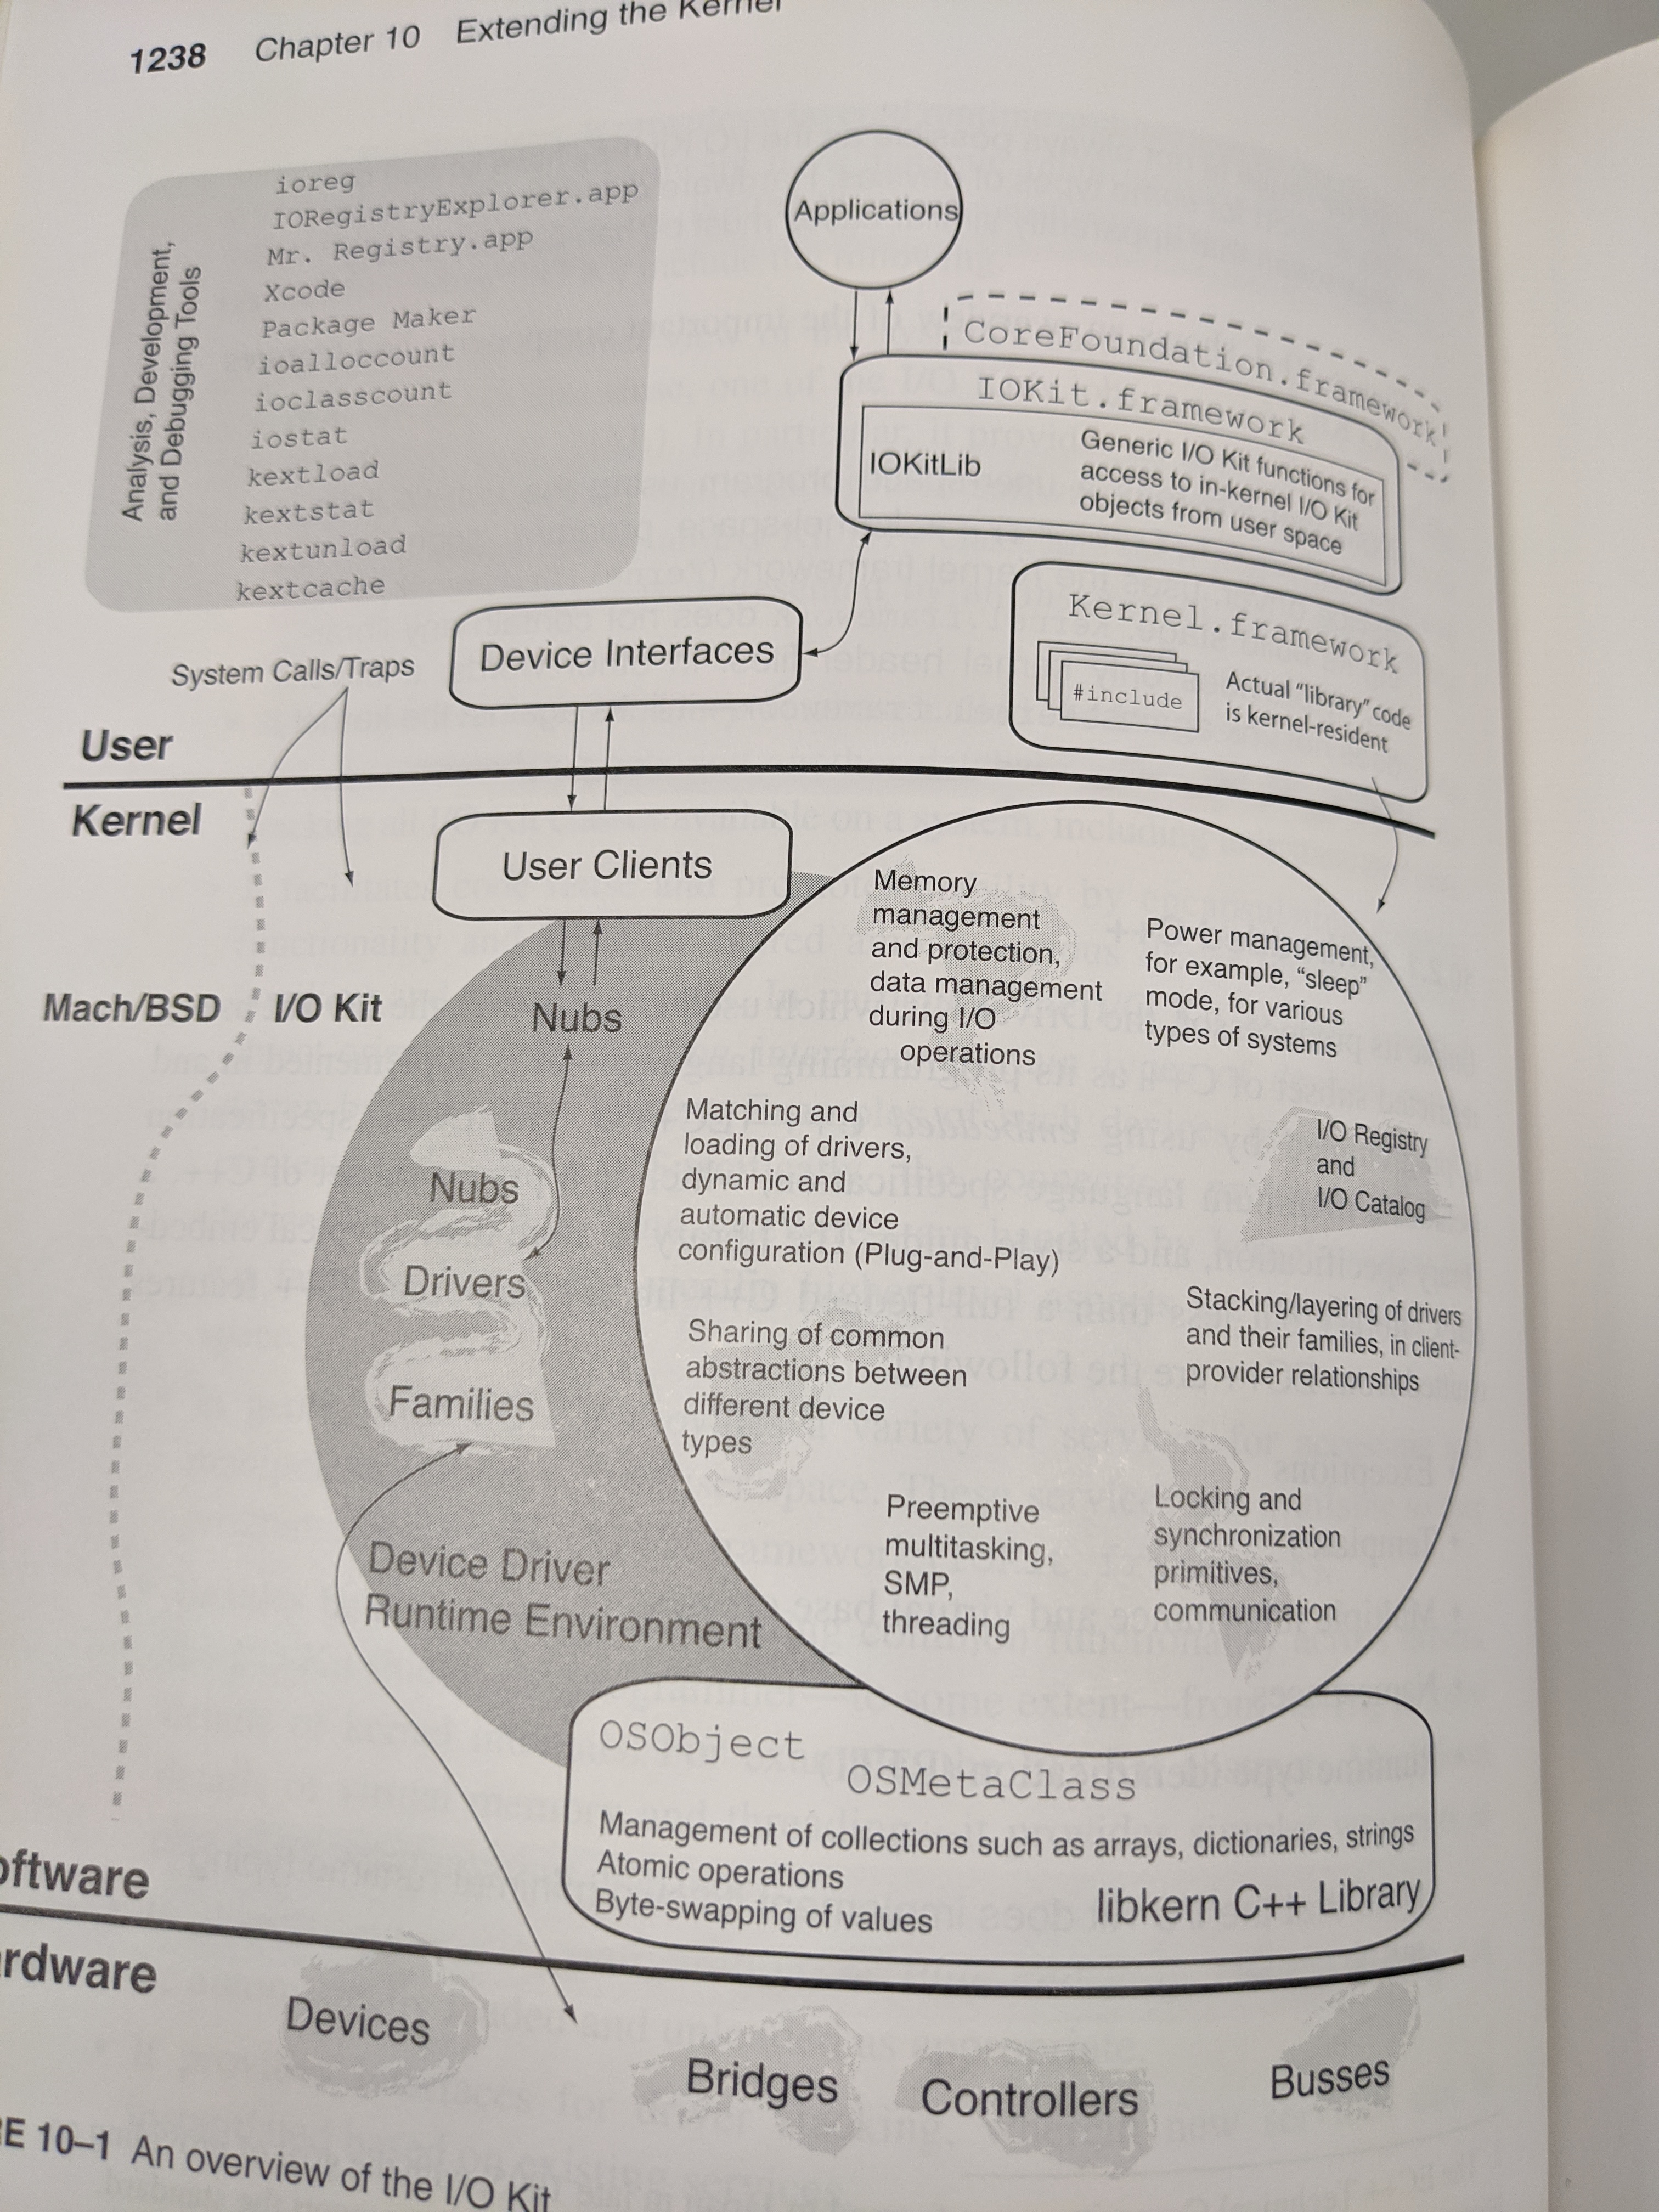
\includegraphics[width=.3\textwidth,keepaspectratio]{iokit-overview.png}
      \caption{Figure from \cite{Singh:2006:MOX:1076423}}
    \end{figure}
  \end{itemize}
\end{frame}

\begin{frame}
  \frametitle{IOKit HIDClass}
  \begin{itemize}
  \item IOKit/IOKit Family/HID class \cite{iokit:family}: Originally it's for USB, but it's far beyond that now. So there is \textbf{Usage Page}.
    \item a command line tool that can be used to enumrate IOKit devices is \texttt{ioreg(8)}
    \begin{figure}
      \includegraphics[width=\textwidth,keepaspectratio]{ioreg-1.png}
      \caption{AppleEmbeddedNVMeTemperatureSensor shown by \texttt{ioreg -l}}
    \end{figure}
    \item you can see \texttt{"PrimaryUsage" = 5}, \texttt{"PrimaryUsagePage" = 65280}, and \texttt{"DeviceUsagePairs" = ({"DeviceUsagePage"=65280,"DeviceUsage"=5})}
  \end{itemize}
\end{frame}

\begin{frame}
  \frametitle{Build the App}
  \begin{itemize}
  \item if you \texttt{git clone} the source code and try to build it, you will get error message saying IOKit related header can't be found (of course, you know you have to change signing stuff)
  \item you have to borrow them from macOS SDK,
    \begin{enumerate}
    \item \texttt{pushd .}
    \item \texttt{cd \path{/Applications/Xcode.app/Contents/Developer/Platforms/iPhoneOS.platform/Developer/SDKs/iPhoneOS.sdk/System/Library/Frameworks/IOKit.framework/}}
    \item \texttt{sudo ln -s \path{/Applications/Xcode.app/Contents/Developer/Platforms/MacOSX.platform/Developer/SDKs/MacOSX.sdk/System/Library/Frameworks/IOKit.framework/Headers} .}
    \item \texttt{popd}
    \end{enumerate}
  \end{itemize}
\end{frame}

\begin{frame}
  \frametitle{AppleHIDUsage}
  \begin{itemize}
  \item \href{https://opensource.apple.com/source/IOHIDFamily/IOHIDFamily-701.60.2/IOHIDFamily/AppleHIDUsageTables.h.auto.html}{AppleHIDUsageTables}
    \item \href{https://opensource.apple.com/source/IOHIDFamily/IOHIDFamily-701.60.2/IOHIDFamily/IOHIDEventTypes.h.auto.html}{IOHIDEventTypes}
  \end{itemize}
\end{frame}

\section{More Thermal Control Related Mechanisms}
\begin{frame}[allowframebreaks]
  \frametitle{More Thermal Control Related Mechanisms}
  \begin{itemize}
  \item There is \path{/usr/libexec/thermalmonitord} in iOS 13 (\path{/usr/libexec/mobilewatchdog} in iOS 12.x), which collects thermal information and does thermal-throttling when necessary.
  \item The thermalmonitord is mainly written in Objective-C (how to know that? there are Objective-C sections in Mach-O).
  \item Mach-O has been around for more than 30 years.There are many tools we can used to inspect Mach-O files. E.g., if you know binutils, llvm-based binutils.
  \item \texttt{class-dump}, one of the interesting Mach-O tools, could extract Objective-C class related information (including protocols and methods) from Mach-O files and convert those them to Objective-C headers.
    \begin{itemize}
    \item \texttt{class-dump thermalmonitord} of iPhone 8 running iOS 13.3 (\texttt{class-dump thermalmonitord -H -o /tmp/thermal\_headers}), we can get more than 100 headers.
    \end{itemize}
  \item How about runtime infomation? So far, I think \texttt{cycript} \cite{cycript} is the most convenient tool if you are willing to learn a new language.
  \end{itemize}
\end{frame}

\begin{frame}
  \begin{figure}
    \includegraphics[height=.8\textheight,keepaspectratio]{ios-thermal-manager.pdf}
    \caption{iOS Thermal Manager}
  \end{figure}
\end{frame}

\begin{frame}
  \begin{figure}
    \includegraphics[height=.8\textheight,keepaspectratio]{ios-thermal-manager-more.pdf}
    \caption{iOS Thermal Manager and others}
  \end{figure}
\end{frame}

\begin{frame}
  \begin{figure}
    \includegraphics[width=.8\textwidth,keepaspectratio]{iOS-thermal.pdf}
    \caption{Example iOS Thermal Control Loops}
  \end{figure}
\end{frame}

\begin{frame}
  \frametitle{Yes, PID control is used}
  \begin{figure}
    \includegraphics[width=.8\textwidth,keepaspectratio]{PID_en.png}
    \caption{PID figure from Wikipedia, \url{https://en.wikipedia.org/wiki/PID_controller}}
  \end{figure}
\end{frame}


\begin{frame}[allowframebreaks]
  \frametitle{peeking running systems with cycript}
  \begin{itemize}
  \item attaching cycript to a running system process is a bit more complicated after iOS 12. We could start from a wrapper called cycrun, \url{https://www.reddit.com/r/jailbreakdevelopers/comments/b1r5kq/question\_is\_cycript\_coming\_to\_ios\_12\_unc0ver\_jb/}
  \item with \texttt{cyrun+cycript},
  \item \texttt{cyrun -x thermalmonitord -e}
  \item then where to start, singleton ones are less intrusive and easier
    \begin{figure}
      \includegraphics[width=.8\textwidth,keepaspectratio]{cycript-1.png}
      \caption{TGraphSample}
    \end{figure}
    \item as you see, we can get \texttt{productObj}
      \begin{figure}
        \includegraphics[width=.8\textwidth,keepaspectratio]{cycript-2.png}
        \caption{HidSensors}
      \end{figure}
      \item as you can see, the \texttt{thermalmonitord} uses HID sensors.
  \end{itemize}
\end{frame}

\section{Other Tools}
\begin{frame}
  \frametitle{Other tools}
  \begin{itemize}
  \item binutils and other hacking tools, such as lsof
  \item lldb/gdb on devices: Apple used to ship ``fat'' gdb and lldb, but not anymore(?). LLDB allows using Objective-C style syntax (most iOS programmers before Swift was introduced know Objective-C)
  \item remote debbuging: either cross building or native building of lldb could be an ostacle, if you are not afraind of using remote debugging, they (debuggserver and lldb) are open source too.
  \end{itemize}
\end{frame}

\begin{frame}
  \frametitle{template}
  \begin{itemize}
  \item iOS uses many open source components and you can use open source tools to explore iDevices.
  \item how about Android devices: as far as I can tell, most Android devices the ``standard'' Linux thermal framework.
  \end{itemize}
\end{frame}

\begin{frame}[allowframebreaks]
  \begin{block}{References}
    \tiny
    \bibliography{ref}
    \bibliographystyle{acm}
  \end{block} 
\end{frame}

\end{document}
